\let\RaggedRight\raggedright
\let\raggedright\relax
\documentclass[utf8,9pt,mathserif,usepdftitle=false]{beamer}

\usepackage{graphicx}%
\usepackage{float}%
\usepackage{wrapfig}%

\let\RaggedRight\raggedright
\let\raggedright\relax
\documentclass[utf8,9pt,mathserif,usepdftitle=false]{beamer}

\usepackage{graphicx}%
\usepackage{float}%
\usepackage{wrapfig}%

\let\RaggedRight\raggedright
\let\raggedright\relax
\documentclass[utf8,9pt,mathserif,usepdftitle=false]{beamer}

\usepackage{graphicx}%
\usepackage{float}%
\usepackage{wrapfig}%

\let\RaggedRight\raggedright
\let\raggedright\relax
\documentclass[utf8,9pt,mathserif,usepdftitle=false]{beamer}

\usepackage{graphicx}%
\usepackage{float}%
\usepackage{wrapfig}%

\include{present.daf}

% \setbeameroption{show notes on second screen}
\setbeameroption{hide notes}
\mode<presentation>
{
  \usetheme{default}
  %\usecolortheme{default} % dove, beaver
  \usecolortheme{whale}
  %\usefonttheme{serif}
}

\hypersetup{%
  pdfinfo={%
    Title={Защита курсовых работ, ИГУ},%
    Subject={Качественные свойства решений уравнения осцилляций нейтрино в среде},%
    Author={Данеко Илья},%
    Keywords={neutrino oscillation in matter;quality properties}%
  }
}

\title{Качественные свойства решений уравнения осцилляций нейтрино в среде
}%
\author{Данеко И.И.}
\date[ИГУ, 2025]{%
  20 октября 2025\\%
  \vspace*{10ex}%
  \begin{flushright}
    \small
    Научный руководитель: Ломов В.П.\par
  \end{flushright}
  {\vspace*{7ex}
    \footnotesize%
    Иркутск, ФГБОУ ВО ИГУ\par%
  } }

\begin{document}

\begin{frame}
  \titlepage
\end{frame}

\begin{frame}
  \frametitle{Введение}%
  %%%
  % TODO:
  \begin{itemize}
  \item<1->
   Нейтрино — одна из самых необычных частиц в нашем мире.

   \item<2->
   Она обладает нулевым зарядом, полуцелым спином и участвует только в слабом
   взаимодействии.

  \item<3->
  Есть два типа нейтрино: флейворные нейтрино и
  массивные. Первые рождаются, тогда как вторые — распространяются.


  \item<4->%
   В данной работе мы разбираем качественные
  характеристики численного решения уравнения осцилляции нейтрино в среде.
  \end{itemize}
\end{frame}

\begin{frame}

  \frametitle{Осцилляции нейтрино в веществе}%
  %%%
  Уравнение осцилляций в среде
  \begin{equation*}
  	\imath \frac{\partial \Psi}{\partial \xi}=H(\xi)\Psi(\xi).\quad
  \end{equation*}
   \onslide<2->%
  Здесь \({H(\xi)}\) — эрмиртовая матрица
  \begin{equation*}
  	H(\xi)=H_0+\upsilon(\xi)W
  \end{equation*}

   \onslide<3->%
 \(H_{0}\) матрица Гамильтона, которая управляет эволюцией флейвора в вакууме
	\begin{equation*}
		H_{0}=\frac{a}{E}
		\begin{pmatrix}
			0 & 0 & 0\\
			0 & b & 0\\
			0 & 0 & 1
		\end{pmatrix}.
	\end{equation*}
	Здесь \(E\) --- числовое значение энергии нейтрино в МэВ, а
	\(a=4,35196\times10^6\) и \(b=0,030554\) --- безразмерные параметры.

\end{frame}

\begin{frame}

  \frametitle{Осцилляции нейтрино в веществе}%
  %%%


   \onslide<1->%
  Второй член в скобках учитывает эффекты, связанные с когерентным взаимодействием нейтрино с фоновыми частицами. Матрица \(W\) имеет вид:
  \begin{equation*}
  	W=
  	\begin{pmatrix}
  		c_{13}^{2}c_{12}^{2} & c_{12}s_{12}c_{13}^{2} & c_{12}c_{13}s_{13}\\
  		c_{12}s_{12}c_{13}^{2} & s_{12}^{2}c_{13}^{2} & s_{12}c_{13}s_{13}\\
  		c_{12}s_{13}c_{13} & s_{12}c_{13}s_{13} & s_{13}^{2}
  	\end{pmatrix}.
  \end{equation*}

  \onslide<2->%
  Профиль плотности для солнечной модели

  \begin{equation*}
  	\upsilon(\xi)=\gamma \exp^{-\eta\xi}
  \end{equation*}

  \onslide<3->%
Начальное состояние мы взяли соответствующие электронному нейтрино
  \begin{equation*}
  		\Psi(\xi_0)=
  	\begin{pmatrix}
  		c_{13}c_{12}\\
  		 s_{12}c_{13}\\
  		 s_{13}
	\end{pmatrix}.
  \end{equation*}
\end{frame}

\begin{frame}
	\frametitle{Качественные свойства решения}%
	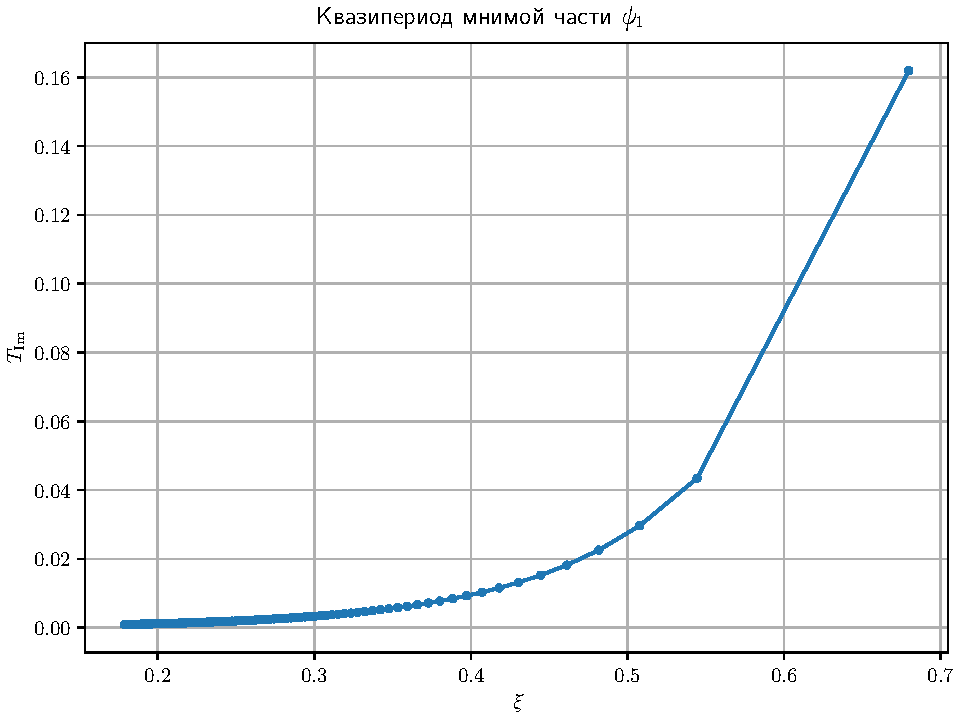
\includegraphics[width=\linewidth]{Ipsi1_width-ru}
\end{frame}


\begin{frame}
	\frametitle{Качественные свойства решения}%
	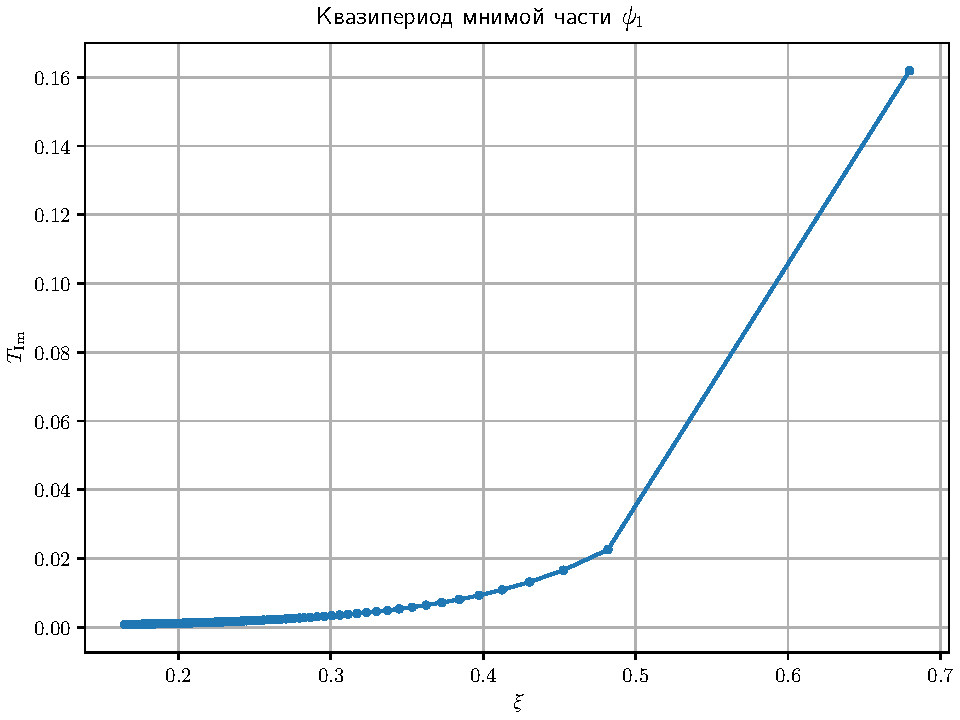
\includegraphics[width=\linewidth]{../../data/magexp/figs/Ipsi1_width-ru}
\end{frame}

\begin{frame}
  \frametitle{Заключение}%
  %%%
  Мы разработали и проверили схему получения качественных характеристик численного
решения уравнения осцилляции нейтрино в среде. Проверили её и при использовании метода Дормана-Принса, и при использовании метода M4.
Проверка показала, что применяемый алгоритм не всегда дают достаточно точный результат. 
Иногда он порождает выбросы. Но если отбросить выбросы мы получем алгоритм, что находит 
качественные характеристики численного решения

  \begin{itemize}
  \onslide<2->%
  \item<1-> .......................................................

  \onslide<3->%
  \item<2->.......................................................
  \end{itemize}
\end{frame}

\begin{frame}
  \frametitle{КОНЕЦ}%
  \LARGE%
  \centering%
  \bfseries%
  СПАСИБО ЗА ВНИМАНИЕ%
\end{frame}

\end{document}

%%% Local Variables:
%%% mode: latex
%%% fill-column: 80
%%% TeX-master: t
%%% TeX-PDF-mode: t
%%% End:
%%% vim: syn=tex ft=tex tw=80 ts=2 sw=2 et:


% \setbeameroption{show notes on second screen}
\setbeameroption{hide notes}
\mode<presentation>
{
  \usetheme{default}
  %\usecolortheme{default} % dove, beaver
  \usecolortheme{whale}
  %\usefonttheme{serif}
}

\hypersetup{%
  pdfinfo={%
    Title={Защита курсовых работ, ИГУ},%
    Subject={Качественные свойства решений уравнения осцилляций нейтрино в среде},%
    Author={Данеко Илья},%
    Keywords={neutrino oscillation in matter;quality properties}%
  }
}

\title{Качественные свойства решений уравнения осцилляций нейтрино в среде
}%
\author{Данеко И.И.}
\date[ИГУ, 2025]{%
  20 октября 2025\\%
  \vspace*{10ex}%
  \begin{flushright}
    \small
    Научный руководитель: Ломов В.П.\par
  \end{flushright}
  {\vspace*{7ex}
    \footnotesize%
    Иркутск, ФГБОУ ВО ИГУ\par%
  } }

\begin{document}

\begin{frame}
  \titlepage
\end{frame}

\begin{frame}
  \frametitle{Введение}%
  %%%
  % TODO:
  \begin{itemize}
  \item<1->
   Нейтрино — одна из самых необычных частиц в нашем мире.

   \item<2->
   Она обладает нулевым зарядом, полуцелым спином и участвует только в слабом
   взаимодействии.

  \item<3->
  Есть два типа нейтрино: флейворные нейтрино и
  массивные. Первые рождаются, тогда как вторые — распространяются.


  \item<4->%
   В данной работе мы разбираем качественные
  характеристики численного решения уравнения осцилляции нейтрино в среде.
  \end{itemize}
\end{frame}

\begin{frame}

  \frametitle{Осцилляции нейтрино в веществе}%
  %%%
  Уравнение осцилляций в среде
  \begin{equation*}
  	\imath \frac{\partial \Psi}{\partial \xi}=H(\xi)\Psi(\xi).\quad
  \end{equation*}
   \onslide<2->%
  Здесь \({H(\xi)}\) — эрмиртовая матрица
  \begin{equation*}
  	H(\xi)=H_0+\upsilon(\xi)W
  \end{equation*}

   \onslide<3->%
 \(H_{0}\) матрица Гамильтона, которая управляет эволюцией флейвора в вакууме
	\begin{equation*}
		H_{0}=\frac{a}{E}
		\begin{pmatrix}
			0 & 0 & 0\\
			0 & b & 0\\
			0 & 0 & 1
		\end{pmatrix}.
	\end{equation*}
	Здесь \(E\) --- числовое значение энергии нейтрино в МэВ, а
	\(a=4,35196\times10^6\) и \(b=0,030554\) --- безразмерные параметры.

\end{frame}

\begin{frame}

  \frametitle{Осцилляции нейтрино в веществе}%
  %%%


   \onslide<1->%
  Второй член в скобках учитывает эффекты, связанные с когерентным взаимодействием нейтрино с фоновыми частицами. Матрица \(W\) имеет вид:
  \begin{equation*}
  	W=
  	\begin{pmatrix}
  		c_{13}^{2}c_{12}^{2} & c_{12}s_{12}c_{13}^{2} & c_{12}c_{13}s_{13}\\
  		c_{12}s_{12}c_{13}^{2} & s_{12}^{2}c_{13}^{2} & s_{12}c_{13}s_{13}\\
  		c_{12}s_{13}c_{13} & s_{12}c_{13}s_{13} & s_{13}^{2}
  	\end{pmatrix}.
  \end{equation*}

  \onslide<2->%
  Профиль плотности для солнечной модели

  \begin{equation*}
  	\upsilon(\xi)=\gamma \exp^{-\eta\xi}
  \end{equation*}

  \onslide<3->%
Начальное состояние мы взяли соответствующие электронному нейтрино
  \begin{equation*}
  		\Psi(\xi_0)=
  	\begin{pmatrix}
  		c_{13}c_{12}\\
  		 s_{12}c_{13}\\
  		 s_{13}
	\end{pmatrix}.
  \end{equation*}
\end{frame}

\begin{frame}
	\frametitle{Качественные свойства решения}%
	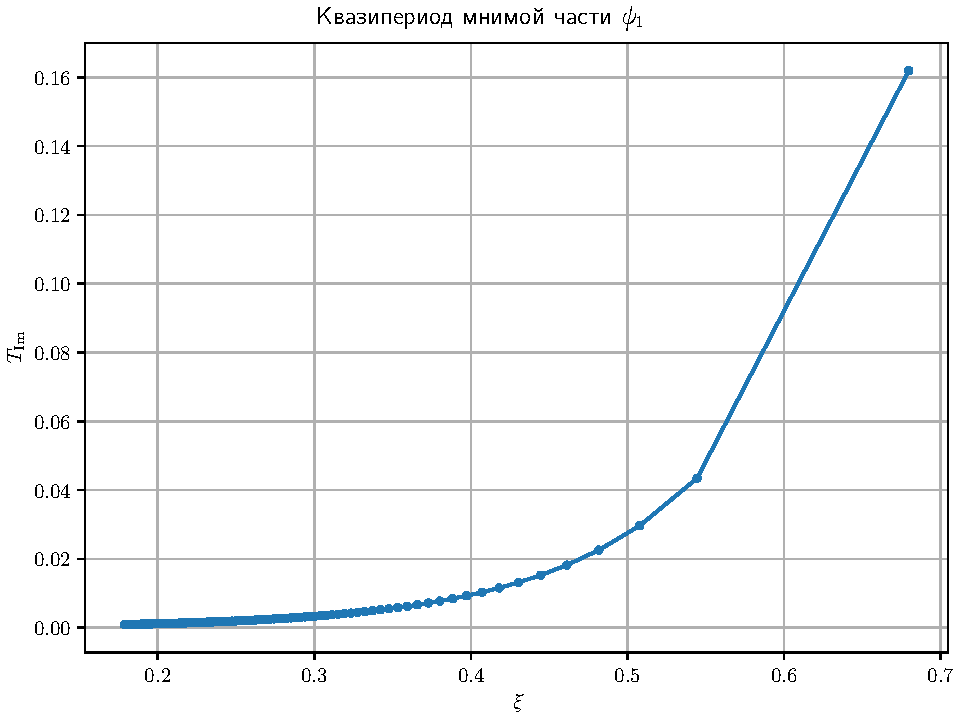
\includegraphics[width=\linewidth]{Ipsi1_width-ru}
\end{frame}


\begin{frame}
	\frametitle{Качественные свойства решения}%
	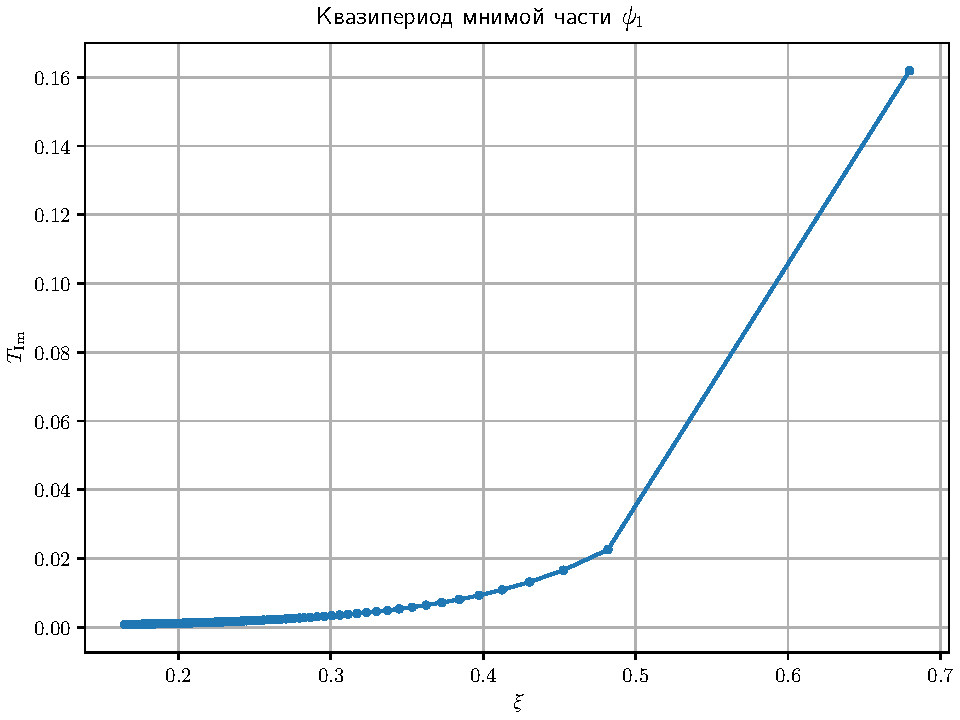
\includegraphics[width=\linewidth]{../../data/magexp/figs/Ipsi1_width-ru}
\end{frame}

\begin{frame}
  \frametitle{Заключение}%
  %%%
  Мы разработали и проверили схему получения качественных характеристик численного
решения уравнения осцилляции нейтрино в среде. Проверили её и при использовании метода Дормана-Принса, и при использовании метода M4.
Проверка показала, что применяемый алгоритм не всегда дают достаточно точный результат. 
Иногда он порождает выбросы. Но если отбросить выбросы мы получем алгоритм, что находит 
качественные характеристики численного решения

  \begin{itemize}
  \onslide<2->%
  \item<1-> .......................................................

  \onslide<3->%
  \item<2->.......................................................
  \end{itemize}
\end{frame}

\begin{frame}
  \frametitle{КОНЕЦ}%
  \LARGE%
  \centering%
  \bfseries%
  СПАСИБО ЗА ВНИМАНИЕ%
\end{frame}

\end{document}

%%% Local Variables:
%%% mode: latex
%%% fill-column: 80
%%% TeX-master: t
%%% TeX-PDF-mode: t
%%% End:
%%% vim: syn=tex ft=tex tw=80 ts=2 sw=2 et:


% \setbeameroption{show notes on second screen}
\setbeameroption{hide notes}
\mode<presentation>
{
  \usetheme{default}
  %\usecolortheme{default} % dove, beaver
  \usecolortheme{whale}
  %\usefonttheme{serif}
}

\hypersetup{%
  pdfinfo={%
    Title={Защита курсовых работ, ИГУ},%
    Subject={Качественные свойства решений уравнения осцилляций нейтрино в среде},%
    Author={Данеко Илья},%
    Keywords={neutrino oscillation in matter;quality properties}%
  }
}

\title{Качественные свойства решений уравнения осцилляций нейтрино в среде
}%
\author{Данеко И.И.}
\date[ИГУ, 2025]{%
  20 октября 2025\\%
  \vspace*{10ex}%
  \begin{flushright}
    \small
    Научный руководитель: Ломов В.П.\par
  \end{flushright}
  {\vspace*{7ex}
    \footnotesize%
    Иркутск, ФГБОУ ВО ИГУ\par%
  } }

\begin{document}

\begin{frame}
  \titlepage
\end{frame}

\begin{frame}
  \frametitle{Введение}%
  %%%
  % TODO:
  \begin{itemize}
  \item<1->
   Нейтрино — одна из самых необычных частиц в нашем мире.

   \item<2->
   Она обладает нулевым зарядом, полуцелым спином и участвует только в слабом
   взаимодействии.

  \item<3->
  Есть два типа нейтрино: флейворные нейтрино и
  массивные. Первые рождаются, тогда как вторые — распространяются.


  \item<4->%
   В данной работе мы разбираем качественные
  характеристики численного решения уравнения осцилляции нейтрино в среде.
  \end{itemize}
\end{frame}

\begin{frame}

  \frametitle{Осцилляции нейтрино в веществе}%
  %%%
  Уравнение осцилляций в среде
  \begin{equation*}
  	\imath \frac{\partial \Psi}{\partial \xi}=H(\xi)\Psi(\xi).\quad
  \end{equation*}
   \onslide<2->%
  Здесь \({H(\xi)}\) — эрмиртовая матрица
  \begin{equation*}
  	H(\xi)=H_0+\upsilon(\xi)W
  \end{equation*}

   \onslide<3->%
 \(H_{0}\) матрица Гамильтона, которая управляет эволюцией флейвора в вакууме
	\begin{equation*}
		H_{0}=\frac{a}{E}
		\begin{pmatrix}
			0 & 0 & 0\\
			0 & b & 0\\
			0 & 0 & 1
		\end{pmatrix}.
	\end{equation*}
	Здесь \(E\) --- числовое значение энергии нейтрино в МэВ, а
	\(a=4,35196\times10^6\) и \(b=0,030554\) --- безразмерные параметры.

\end{frame}

\begin{frame}

  \frametitle{Осцилляции нейтрино в веществе}%
  %%%


   \onslide<1->%
  Второй член в скобках учитывает эффекты, связанные с когерентным взаимодействием нейтрино с фоновыми частицами. Матрица \(W\) имеет вид:
  \begin{equation*}
  	W=
  	\begin{pmatrix}
  		c_{13}^{2}c_{12}^{2} & c_{12}s_{12}c_{13}^{2} & c_{12}c_{13}s_{13}\\
  		c_{12}s_{12}c_{13}^{2} & s_{12}^{2}c_{13}^{2} & s_{12}c_{13}s_{13}\\
  		c_{12}s_{13}c_{13} & s_{12}c_{13}s_{13} & s_{13}^{2}
  	\end{pmatrix}.
  \end{equation*}

  \onslide<2->%
  Профиль плотности для солнечной модели

  \begin{equation*}
  	\upsilon(\xi)=\gamma \exp^{-\eta\xi}
  \end{equation*}

  \onslide<3->%
Начальное состояние мы взяли соответствующие электронному нейтрино
  \begin{equation*}
  		\Psi(\xi_0)=
  	\begin{pmatrix}
  		c_{13}c_{12}\\
  		 s_{12}c_{13}\\
  		 s_{13}
	\end{pmatrix}.
  \end{equation*}
\end{frame}

\begin{frame}
	\frametitle{Качественные свойства решения}%
	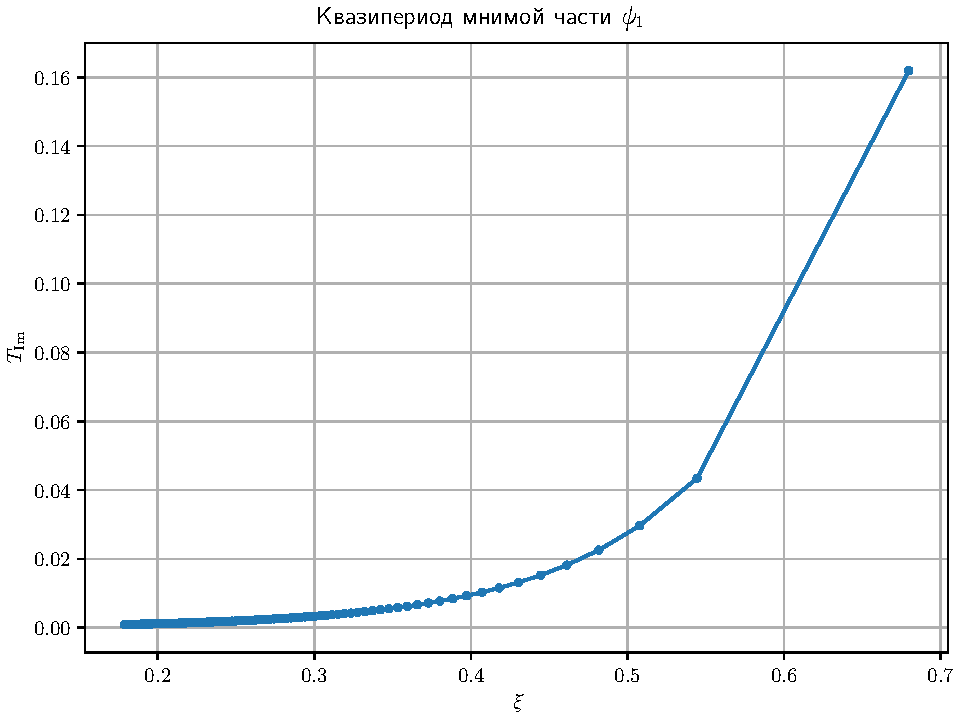
\includegraphics[width=\linewidth]{Ipsi1_width-ru}
\end{frame}


\begin{frame}
	\frametitle{Качественные свойства решения}%
	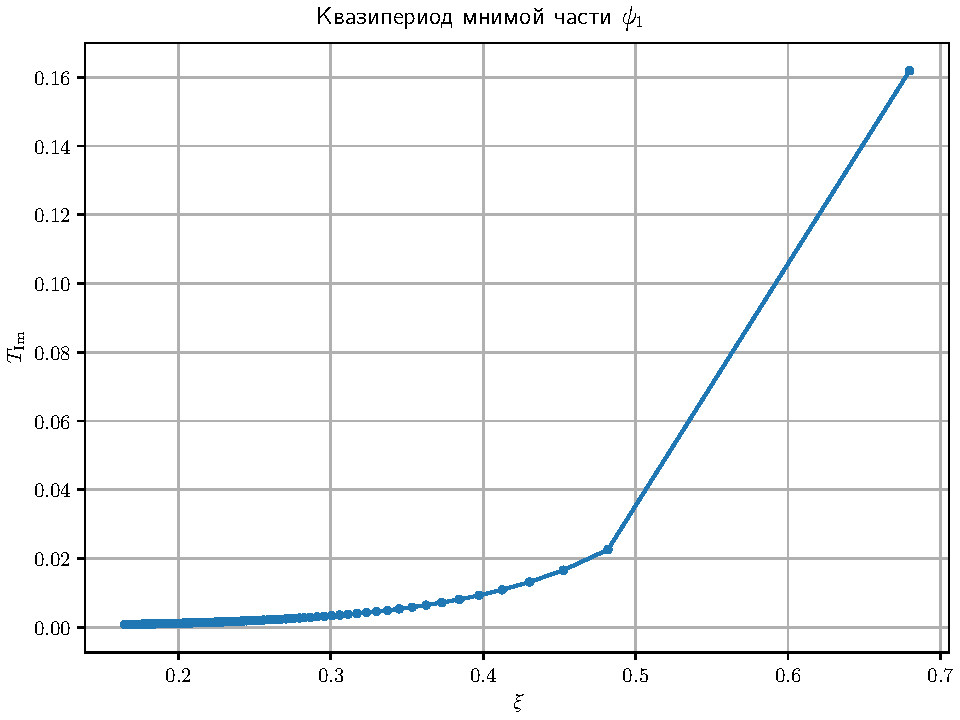
\includegraphics[width=\linewidth]{../../data/magexp/figs/Ipsi1_width-ru}
\end{frame}

\begin{frame}
  \frametitle{Заключение}%
  %%%
  Мы разработали и проверили схему получения качественных характеристик численного
решения уравнения осцилляции нейтрино в среде. Проверили её и при использовании метода Дормана-Принса, и при использовании метода M4.
Проверка показала, что применяемый алгоритм не всегда дают достаточно точный результат. 
Иногда он порождает выбросы. Но если отбросить выбросы мы получем алгоритм, что находит 
качественные характеристики численного решения

  \begin{itemize}
  \onslide<2->%
  \item<1-> .......................................................

  \onslide<3->%
  \item<2->.......................................................
  \end{itemize}
\end{frame}

\begin{frame}
  \frametitle{КОНЕЦ}%
  \LARGE%
  \centering%
  \bfseries%
  СПАСИБО ЗА ВНИМАНИЕ%
\end{frame}

\end{document}

%%% Local Variables:
%%% mode: latex
%%% fill-column: 80
%%% TeX-master: t
%%% TeX-PDF-mode: t
%%% End:
%%% vim: syn=tex ft=tex tw=80 ts=2 sw=2 et:


% \setbeameroption{show notes on second screen}
\setbeameroption{hide notes}
\mode<presentation>
{
  \usetheme{default}
  %\usecolortheme{default} % dove, beaver
  \usecolortheme{whale}
  %\usefonttheme{serif}
}

\hypersetup{%
  pdfinfo={%
    Title={Защита курсовых работ, ИГУ},%
    Subject={Качественные свойства решений уравнения осцилляций нейтрино в среде},%
    Author={Данеко Илья},%
    Keywords={neutrino oscillation in matter;quality properties}%
  }
}

\title{Качественные свойства решений уравнения осцилляций нейтрино в среде
}%
\author{Данеко И.И.}
\date[ИГУ, 2025]{%
  20 октября 2025\\%
  \vspace*{10ex}%
  \begin{flushright}
    \small
    Научный руководитель: Ломов В.П.\par
  \end{flushright}
  {\vspace*{7ex}
    \footnotesize%
    Иркутск, ФГБОУ ВО ИГУ\par%
  } }

\begin{document}

\begin{frame}
  \titlepage
\end{frame}

\begin{frame}
  \frametitle{Введение}%
  %%%
  % TODO:
  \begin{itemize}
  \item<1->
   Нейтрино — одна из самых необычных частиц в нашем мире.

   \item<2->
   Она обладает нулевым зарядом, полуцелым спином и участвует только в слабом
   взаимодействии.

  \item<3->
  Есть два типа нейтрино: флейворные нейтрино и
  массивные. Первые рождаются, тогда как вторые — распространяются.


  \item<4->%
   В данной работе мы разбираем качественные
  характеристики численного решения уравнения осцилляции нейтрино в среде.
  \end{itemize}
\end{frame}

\begin{frame}

  \frametitle{Осцилляции нейтрино в веществе}%
  %%%
  Уравнение осцилляций в среде
  \begin{equation*}
  	\imath \frac{\partial \Psi}{\partial \xi}=H(\xi)\Psi(\xi).\quad
  \end{equation*}
   \onslide<2->%
  Здесь \({H(\xi)}\) — эрмиртовая матрица
  \begin{equation*}
  	H(\xi)=H_0+\upsilon(\xi)W
  \end{equation*}

   \onslide<3->%
 \(H_{0}\) матрица Гамильтона, которая управляет эволюцией флейвора в вакууме
	\begin{equation*}
		H_{0}=\frac{a}{E}
		\begin{pmatrix}
			0 & 0 & 0\\
			0 & b & 0\\
			0 & 0 & 1
		\end{pmatrix}.
	\end{equation*}
	Здесь \(E\) --- числовое значение энергии нейтрино в МэВ, а
	\(a=4,35196\times10^6\) и \(b=0,030554\) --- безразмерные параметры.

\end{frame}

\begin{frame}

  \frametitle{Осцилляции нейтрино в веществе}%
  %%%


   \onslide<1->%
  Второй член в скобках учитывает эффекты, связанные с когерентным взаимодействием нейтрино с фоновыми частицами. Матрица \(W\) имеет вид:
  \begin{equation*}
  	W=
  	\begin{pmatrix}
  		c_{13}^{2}c_{12}^{2} & c_{12}s_{12}c_{13}^{2} & c_{12}c_{13}s_{13}\\
  		c_{12}s_{12}c_{13}^{2} & s_{12}^{2}c_{13}^{2} & s_{12}c_{13}s_{13}\\
  		c_{12}s_{13}c_{13} & s_{12}c_{13}s_{13} & s_{13}^{2}
  	\end{pmatrix}.
  \end{equation*}

  \onslide<2->%
  Профиль плотности для солнечной модели

  \begin{equation*}
  	\upsilon(\xi)=\gamma \exp^{-\eta\xi}
  \end{equation*}

  \onslide<3->%
Начальное состояние мы взяли соответствующие электронному нейтрино
  \begin{equation*}
  		\Psi(\xi_0)=
  	\begin{pmatrix}
  		c_{13}c_{12}\\
  		 s_{12}c_{13}\\
  		 s_{13}
	\end{pmatrix}.
  \end{equation*}
\end{frame}

\begin{frame}
	\frametitle{Качественные свойства решения}%
	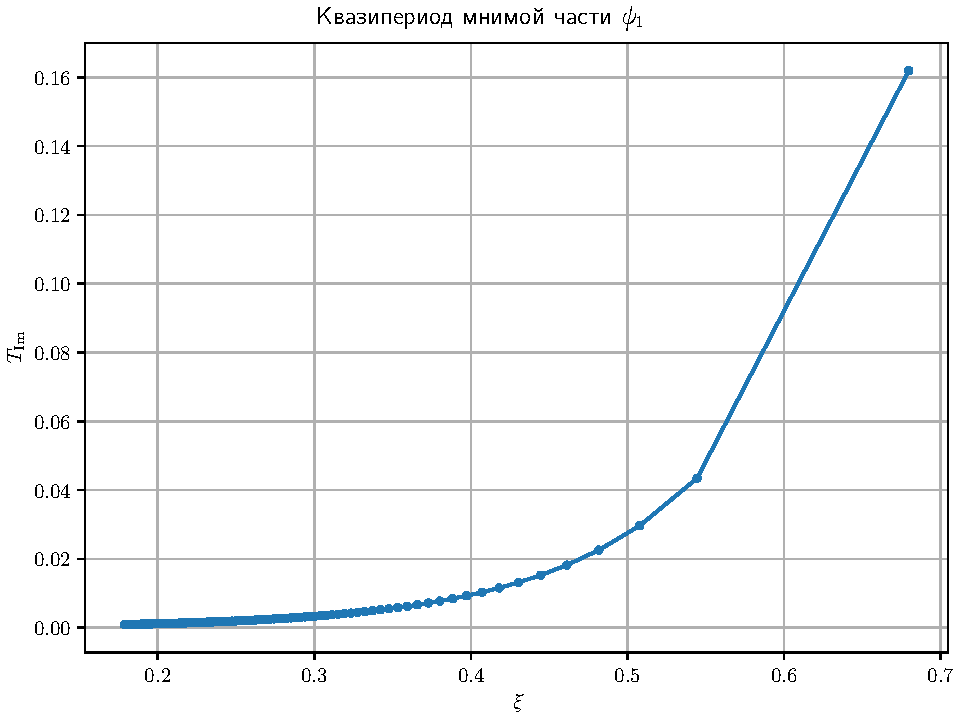
\includegraphics[width=\linewidth]{Ipsi1_width-ru}
\end{frame}


\begin{frame}
	\frametitle{Качественные свойства решения}%
	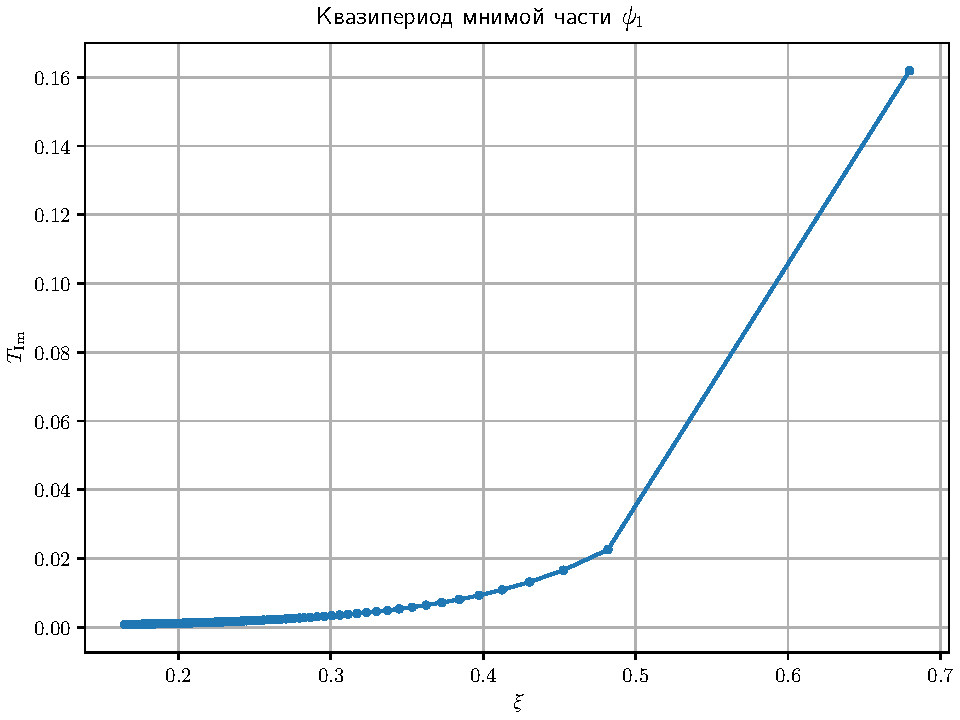
\includegraphics[width=\linewidth]{../../data/magexp/figs/Ipsi1_width-ru}
\end{frame}

\begin{frame}
  \frametitle{Заключение}%
  %%%
  Мы разработали и проверили схему получения качественных характеристик численного
решения уравнения осцилляции нейтрино в среде. Проверили её и при использовании метода Дормана-Принса, и при использовании метода M4.
Проверка показала, что применяемый алгоритм не всегда дают достаточно точный результат. 
Иногда он порождает выбросы. Но если отбросить выбросы мы получем алгоритм, что находит 
качественные характеристики численного решения

  \begin{itemize}
  \onslide<2->%
  \item<1-> .......................................................

  \onslide<3->%
  \item<2->.......................................................
  \end{itemize}
\end{frame}

\begin{frame}
  \frametitle{КОНЕЦ}%
  \LARGE%
  \centering%
  \bfseries%
  СПАСИБО ЗА ВНИМАНИЕ%
\end{frame}

\end{document}

%%% Local Variables:
%%% mode: latex
%%% fill-column: 80
%%% TeX-master: t
%%% TeX-PDF-mode: t
%%% End:
%%% vim: syn=tex ft=tex tw=80 ts=2 sw=2 et:
